\section{Integration}
Disparate hardware timing channel protection mechanisms are not enough to 
implement a full, timing channel secure system. It requires support from 
software to manage the interaction of software entities with the hardware.  
Further, these hardware mechanisms are often interdependent. The shared cache 
miss path involves the cache, bus, and memory controller, all of which require 
timing channel protection. Haphazardly time multiplexing these resources can 
lead to unnecessarily large performance penalties. The integrated system 
requires carefully coordinating the protected resources. The rest of this 
section elaborates on the timing compartment manager, the software entity that 
initializes and manages timing compartments, and then describes how timing 
channel protection mechanisms should be coordinated.

\subsection{The Timing Compartment Manager}
\label{sec:integration_tcm}
The timing compartment manager (TCM) is responsible for initializing and 
managing timing compartments. At system initialization time it informs the 
hardware of the timing compartments present in the system and configures the 
hardware components with the policy. At run time, the TCM tags requests for 
shared hardware resources with the timing compartment ID (TCID) of the TC that 
originated the request. Shared hardware resources then enforce the policy by 
checking the TCID before handling the request. The hardware allows software 
entities within the same compartment to share resources normally, and timing 
compartments can even be allocated multiple cores.

As shown in Figure \ref{fig:arch}, the timing compartments architecture is 
comprised of a set of $n$ cores which share resources. There is no limitation 
on $m$, the number of timing compartments that can reside in the system at one 
time. However, at most $n$ timing compartments can be active (executing on one 
or more physical cores) at a time. If $m>n$, active timing compartments must 
occasionally be switched with inactive ones. The TCM addresses this by context 
switching TCs according toa context switch schedule.

The TCM is implemented as an extension of the trusted software layer, such as 
the OS or hypervisor. It requires functions to handle the initialization
and context switching. It also requires a small address space of its own to 
store the register contents of inactive TCs and a queue of inactive TCs.
The rest of this section describes the hardware TCID storage elemnts controlled 
by the TCM, and then elaborates on how the TCM initializes the system and 
handles context switching.

\subsubsection{TCIDs}
\begin{figure}
    \begin{center}
        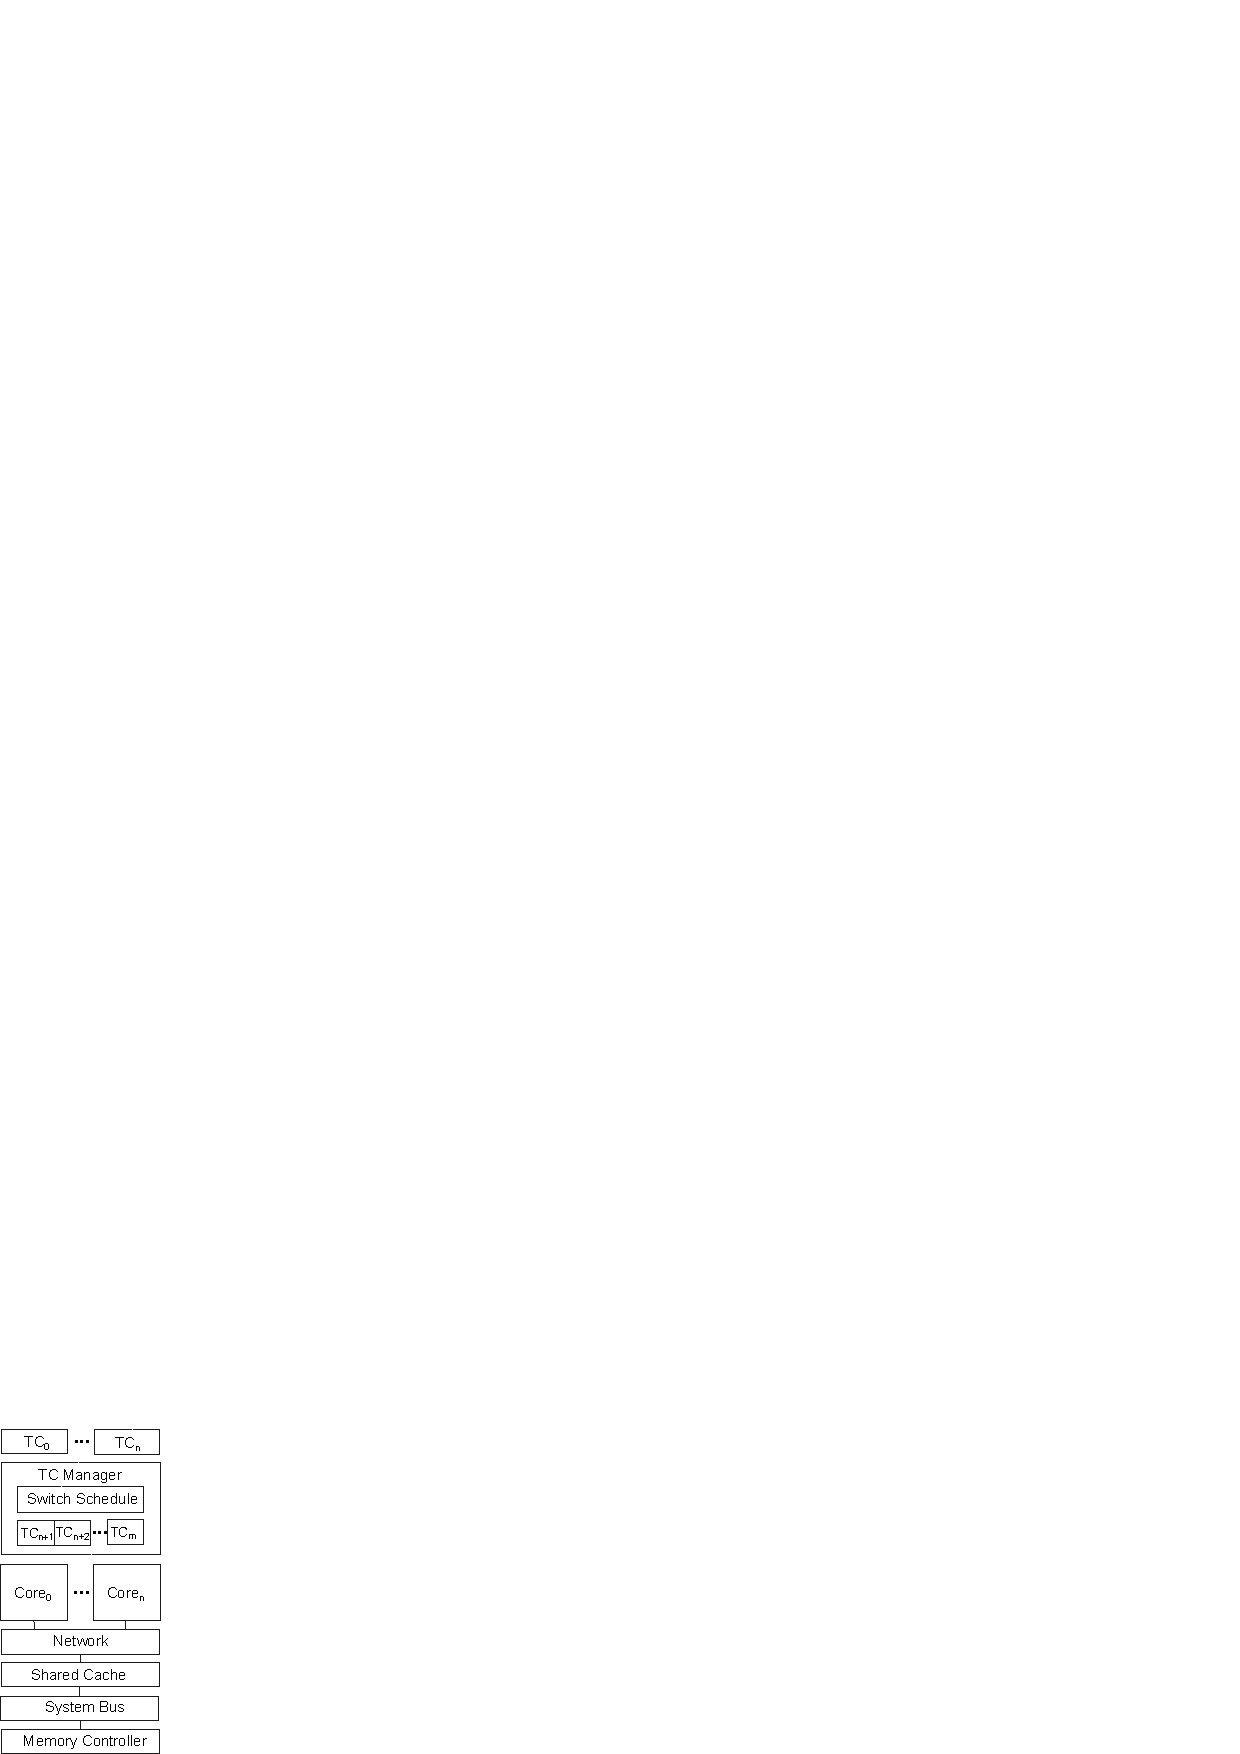
\includegraphics[width=1.08in]{figs/hw_sw_arch.pdf}
        \caption{The Timing Compartments Architecture}
        \label{fig:arch}
    \end{center}
\end{figure}

The hardware protection mechanisms track which timing compartment originated 
each request and handle the requests accordingly. To do so, requests (such as 
network packets or shared cache accesses) are tagged with a timing compartment 
ID (TCID). The set partitioned cache has $n$ registers which store the TCIDs
that own each of the (at most) $n$ partitions. When a request requires a 
replacement, the cache uses the TCID of the request to decide which partitions 
can allow entries to be replaced according to the policy. (Checking is only 
required on replacements since TCIDs have separate address spaces.) Each of the 
separate MSHR banks are tagged with a TCID of the owner, and requests can only 
affect the MSHR banks with the same TCID as the request. Each of the time 
multiplexed resources (the networks, the memory controller, shared cache 
response ports, and memory controller response ports) have $n$ queues. Each of 
these queues has a register to store the TCID which owns that particular queue, 
and time quanta are assigned to each queue. Lastly, each core has a register 
that stores the TCID of the TC currently active on that core. This is used to 
derive the tags that are appended to requests originating from that core. Table 
\ref{table:tcid} summarizes the TCID storage elements in the system.

\begin{table}
    \begin{footnotesize}
\begin{tabular}{l|l}
    \hline
    Component & TCID Storage \\
    \hline
    Core & $n$ cores. TCID register per core. \\
    Shared Cache Port & $n$ queues. TCID register per queue \\
    Shared Cache Partititions & $n$ partition owner registers. \\
    Shared Cache MSHRs & $n$ MSHR banks. TCID per bank \\
    Network & $n$ queues. TCID register per queue\\
    \hline
\end{tabular}
    \end{footnotesize}
    \caption{TCID storage for TC Architecture Components}
    \label{table:tcid}
\end{table}

\subsubsection{Initialization \& Handling Context Switches}
The TCM, initializes the system by setting the TCID storage elements listed in 
Table 1 with the IDs of the initially active timing compartments. At most $n$ 
of these can be active initially, so if $m>n$, some will be inactive, and the 
TCM must define a static context switching schedule at initialization time.

The time between context switches cannot depend on the dynamic behaviour of the 
TCs. Otherwise, a timing compartment could observe the time that they are 
context switched in or out to learn information about the timing compartment it 
is switched with. Instead, context switches occur at a fixed time interval, 
$T_{CTX}$. Every $T_{CTX}$ cycles the TCM is invoked to replace the timing 
compartment which has been active the longest with the TC at the head of the 
inactive TC queue. The compartment which has been switched out is moved to the 
back of the inactive TC queue.

To perform the context switch, the CPU pipeline and the memory request queue 
are drained. The general purpose registers of the outgoing TC are stored in 
TCM-space memory and tagged with the TCID. The private cache, shared cache 
partition, TLB, and branch predictor state of the outgoing TC are all flushed.  
Finally, the TCID stores of the outgoing TC are replaced with the TCID of the 
incoming TC. 

The time required to perform a context switch depends on the state and behavior 
of the outgoing TC. The owner of the incoming TC can observe when the incoming 
TC begins executing, so this implies a potential leakage of secrets.  To 
prevent this, context switches are bound to always take the worst case time.  
If a context switch completes early, the incoming TC is stalled until the worst 
case context switch time has been reached.

\subsection{Coordination}
Naïvely time multiplexing the components with contention based timing channels 
can lead to poor performance since many of these components are on the same 
path to handle a request. 
% During a shared cache miss, the request is sent along the bus that connects 
% the private caches to the shared cache, which we refer to as the L2L3Bus.  
% After detecting the miss, a request is sent to memory through the bus 
% connecting the shared cache to the memory controller, which we refer to as 
% the membus. The memory controller handles the memory request and sends the 
% response back through the membus. Finally, the cache sends a response back 
% through the L2L3Bus.
%%%%%%% The NoC section should mention the request/response layers before this 
%%%%%%% section
On the cache miss path both buses (which are each split into a request and 
response layer), the response ports of the cache and memory controller, and the 
memory controller itself are all time multiplexed. A naïve system design might 
determine an optimal time quantum duration and round robin schedule for each 
resource independently of one another as shown in figure 
\ref{fig:naive_scheme}. The L2-L3 bus is the bus connecting the private caches 
to the shared cache, and the membus connects the shared cache to the memory 
controller.

\begin{figure}
    \begin{center}
        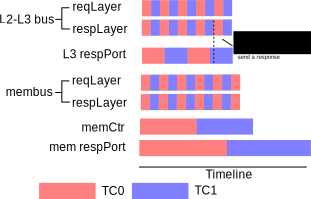
\includegraphics[width=3.46in]{figs/baseline_schedule.pdf}
        \caption{Cache hit timing sequence.}
        \label{fig:naive_scheme}
    \end{center}
\end{figure}

Notably, the time quanta of each component are not aligned with each of the 
L2-L3 bus time quanta.  During a shared cache hit on behalf of $TC1$, 
occasionally the $TC1$ shared cache response port time quantum will be aligned 
with the $TC1$ L2-L3 bus time quantum allowing it to proceed along the path 
without unneeded stalls.  However, sometimes these are not well-aligned and 
$TC1$ will have to wait for $TC2$ to finish before it can proceed. This becomes 
even more wasteful
as the number of timing compartments scales. A request may have to wait through 
each other compartment's time quantum. 

\begin{figure}
    \begin{center}
        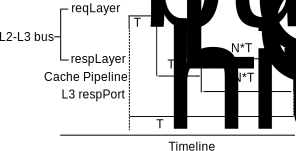
\includegraphics[width=2.4675in]{figs/hit_timing.pdf}
        \caption{Cache hit timing sequence.}
        \label{fig:hit_timing}
    \end{center}
\end{figure}

For ease of analysis, we examine the shared cache hit path before covering the 
complete shared cache miss path. Figure \ref{fig:hit_timing} shows the timing 
of $N$ requests through the shared cache hit path, where $N$ is the number of 
pipeline stages through the fully pipelined cache. Sending a request over the 
L2-L3 bus takes $T_{bus}$ cycles.  The cache then takes $T_{L3L}$ cycles after 
receiving the request before the data for the first of the $N$ requests is 
available to be sent. The response port transfers all the responses in $N\times 
T_{CBT}$ cycles, where $T_{CBT}$ is the time required to transfer a cache block 
over the bus. $T_{hit}$, the total period of the the cache hit timing sequence 
is $T_{bus}+T_{L3L}+N\times T_{CBT}$.

\begin{figure}
    \begin{center}
        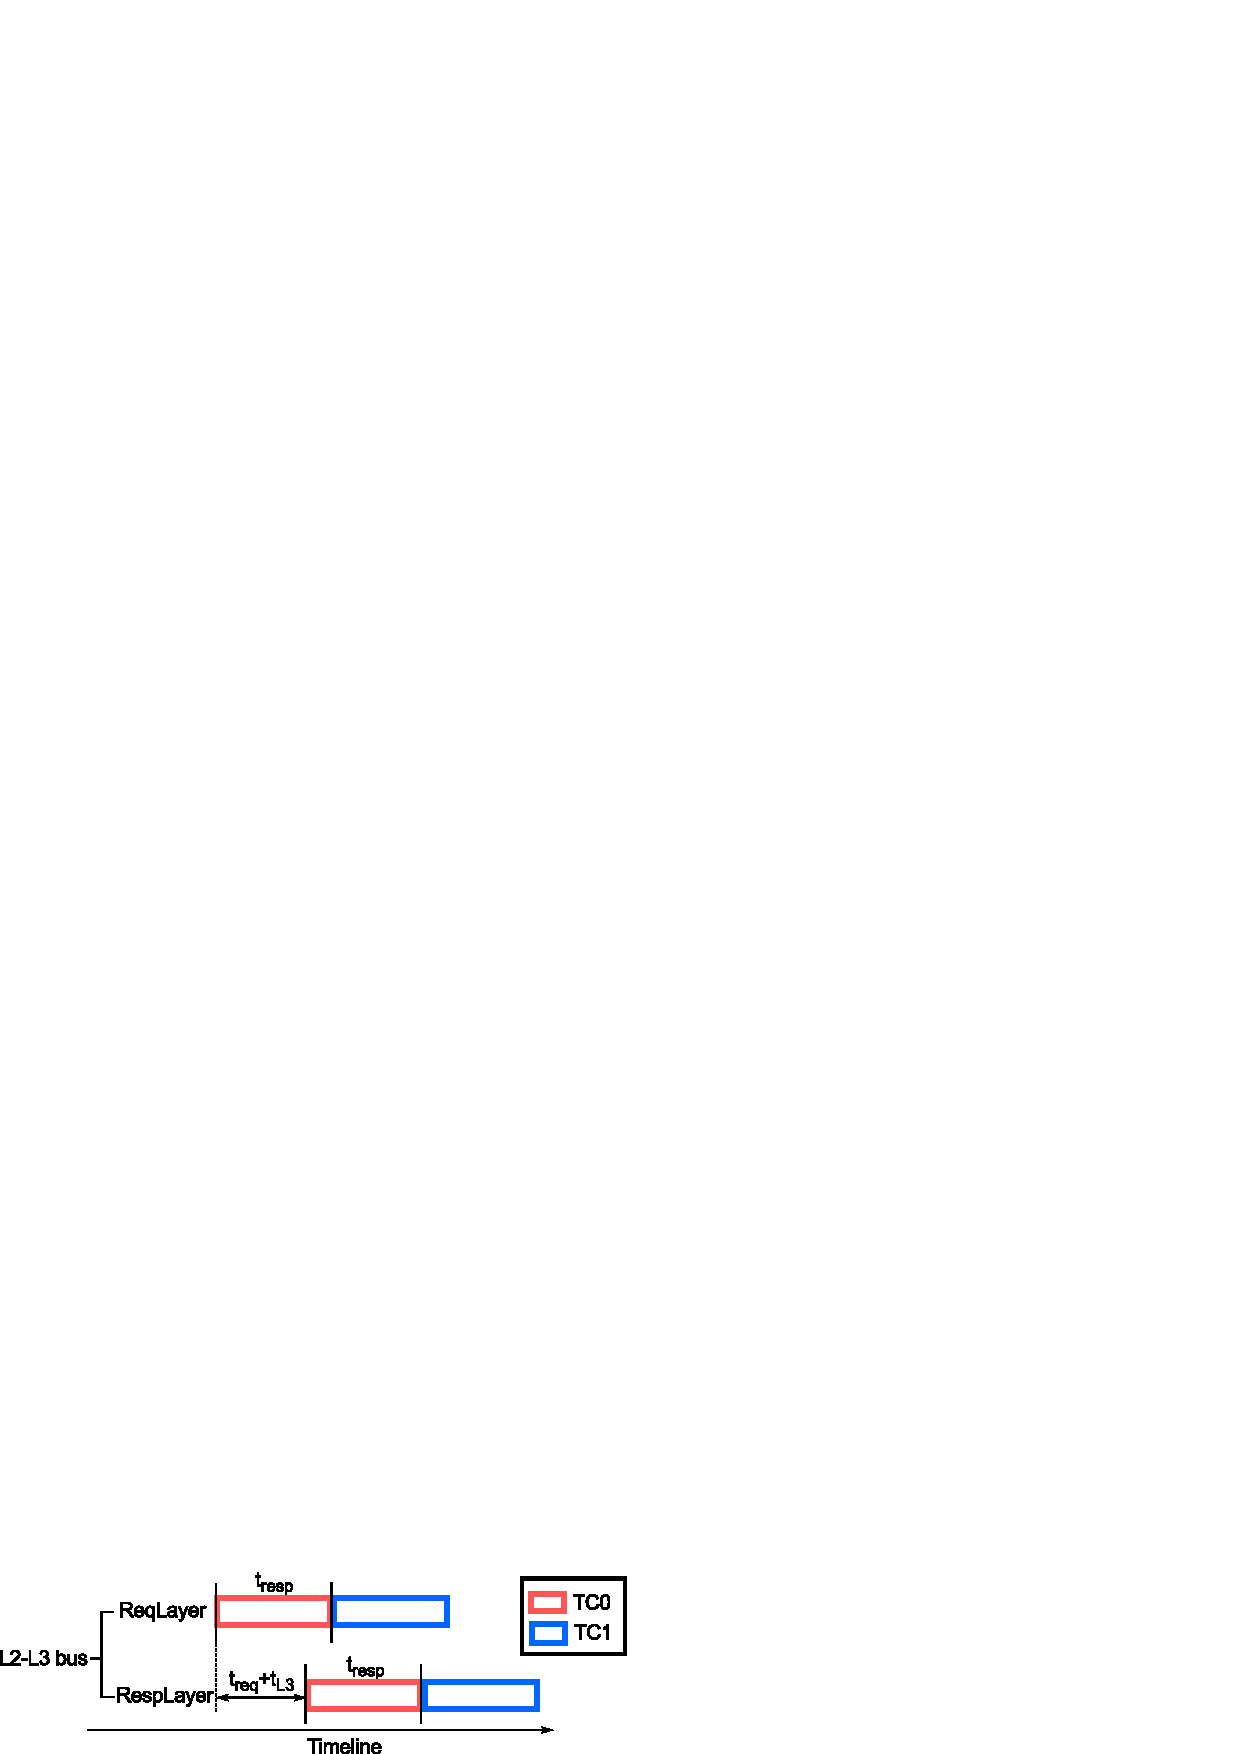
\includegraphics[width=3.2624in]{figs/hit_schedule.pdf}
        \caption{Cache hit timing path schedule.}
        \label{fig:hit_schedule}
    \end{center}
\end{figure}

To improve over the naïve scheme, the schedule must coordinate each of these 
resources to 1) allow a request to proceed through common paths unblocked and 
2) repeat this alignment for each TC. Figure \ref{fig:hit_schedule} shows a 
schedule that allows $N$ requests to proceed unblocked for each TCs turn. The 
time quanta are aligned to follow the timings of \ref{fig:hit_timing}. To 
guarantee that the behavior of a schedule repeats for the time quanta of each 
TC, the durations of the time quanta for each resource must share a common 
factor number of cycles. For example, if $N \times T_{CBT}$ (and this is the 
time quanta duration for the response port and layer) is 16 and $T_{bus}$ is 3, 
the actual time quanta duration for the request layer, $T_{req}$, should be 4, 
8, or 16 even though the request port cannot do useful work for these extra 
cycles. 

\begin{figure}
    \begin{center}
        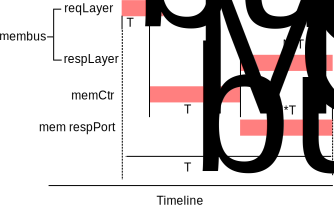
\includegraphics[width=2.9475in]{figs/miss_timing.pdf}
        \caption{The shared cache miss path timing sequence.}
        \label{fig:miss_timing}
    \end{center}
\end{figure}

The analysis for the segment of the shared cache miss path between the shared 
cache and the memory controller is similar. The most significant difference is 
that unlike the cache, the memory controller itself is time multiplexed. Figure 
\ref{fig:miss_timing} shows the timing for this segment of the shared cache 
miss path. The time quanta of the memory controller have a duration that is 
chosen to be $T_{MCL}$. This optimal value may depend on the design, and
the authors of \cite{ushpca14} discuss the selection of this value. $M$ is the 
number of memory requests that can be handled in a single memory controller 
time quantum.
$T_{miss}$, the total period of the cache miss timing sequence is 
$T_{bus}+T_{MCL}+M\times T_{CBT}$.

The schedule of the entire system should allow the shared cache miss path to be 
traversed unblocked.
% , but since cache hits are more frequent than misses, the performance of the 
% cache hit path should not be weakened to meet this goal.
To prevent blocking along the request path, the time quantum of a timing 
compartment on the membus request port should begin just as that timing 
compartment's time quantum on the shared cache memory side request port 
finishes. This prevents blocking along the request path of the membus.
Similarly, to prevent blocking along the response path, the time quantum of the 
shared cache response port should begin just after the time quantum of the same 
timing compartment on the memory bus response layer ends. Figure 
\ref{fig:coordination}
shows a high level view of a full coordinated schedule.

\begin{figure}
    \begin{center}
        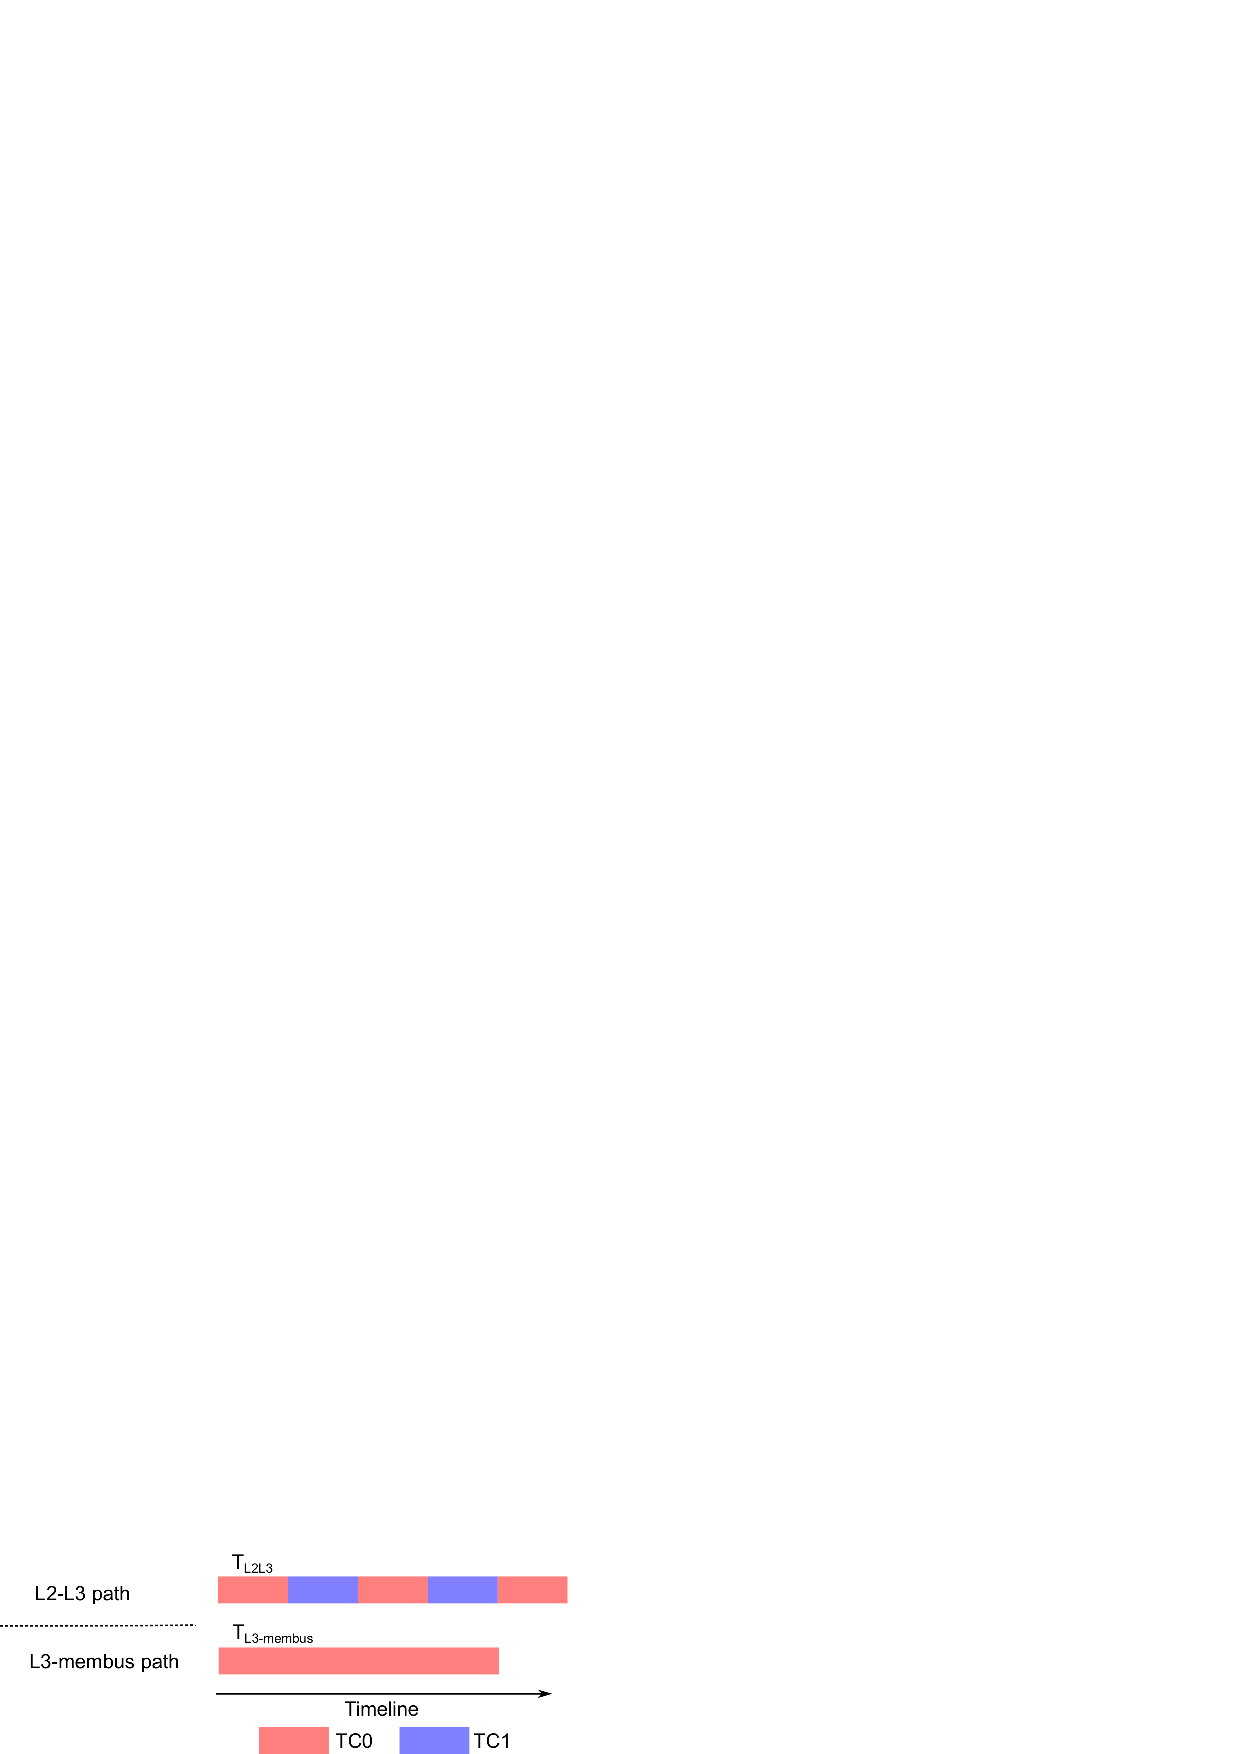
\includegraphics[width=2.9475in]{figs/coordination.pdf}
        \caption{A coordinated cache miss path schedule.}
        \label{fig:coordination}
    \end{center}
\end{figure}

To meet the first criterion, the cache hit path timing sequence shown in 
\ref{fig:hit_timing} should be aligned with the start of the corresponding 
memory bus time quantum. To repeat this behavior for each cache hit path timing 
sequence, $T_{hit}$ and $T_{miss}$
should share a common factor. Since cache 
hits are more frequent than misses, the performance of the cache hit path 
should not be weakened to accomplish this. Instead, the length of the membus 
timing sequence should be increased (e.g. by increasing the memory controller 
time quantum). The second criterion is met if the maximum number of active 
timing compartments in the system (i.e. the number of cores) is a factor of the 
period of the membus timing sequence.
